\chapter{Objetivos}
\label{chap:objetivos}

\drop{H}{oy} en día, la mayor parte de la producción de información en forma de documentos se realiza por medio de herramientas informáticas. Actualmente, en la administración pública se está extendiendo el uso de la firma electrónica, que garantiza la autenticidad del documento digital, pero todavía hay un gran número de personas que no lo utilizan. Es un caso muy habitual que muchos formularios, aún encontrándose en formato digital, se presenten los documentos sobre un soporte físico. %En estos casos para conseguir una gestión eficaz y ágil, es necesario digitalizar previamente estos documentos para incorporarlos al sistema que tenga implementado la organización.
\begin{figure}[h!]
  \begin{center}
      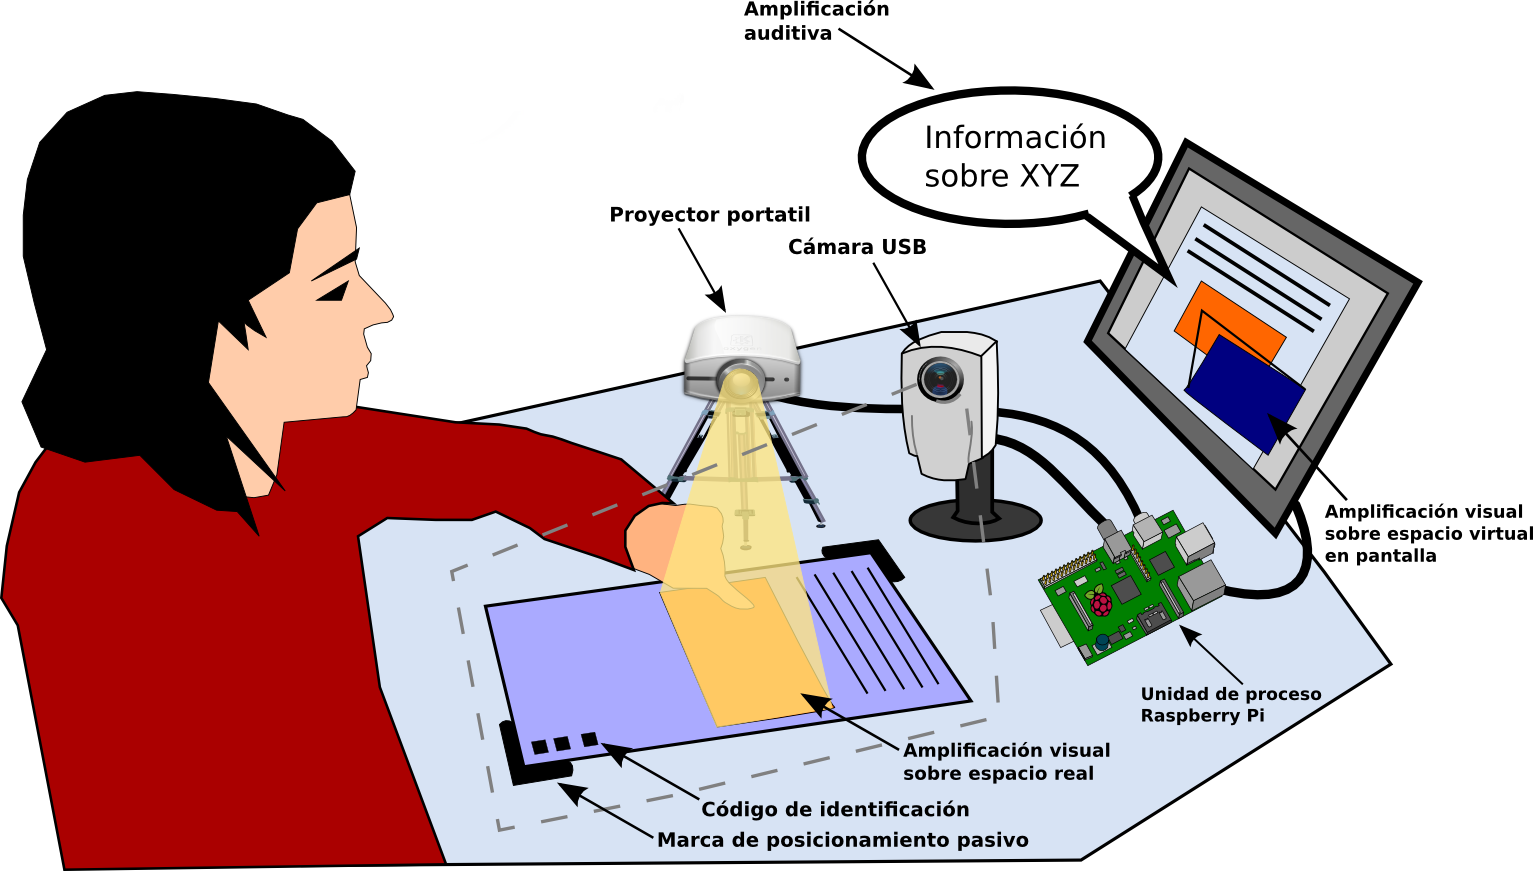
\includegraphics[width=0.85\textwidth]{argos.png}
      \caption{Esquema de componentes funcionales de ARgos}
      \label{fig:diagrama_argos}
    \end{center}
\end{figure}
   
Según lo anterior, sería deseable disponer de una herramienta que permitiera el tratamiento directo sobre estos documentos «físicos». \textit{ARgos} es, un proyecto de la Cátedra INDRA-UCLM que pretende la construcción de un sistema de ayuda a la gestión de documentos impresos mediante el uso de técnicas de visión por computador, síntesis visual y auditiva y técnicas de realidad aumentada. En la figura \ref{fig:diagrama_argos} se recogen los componentes funcionales del sistema.


%\subsection{Objetivos específicos}
GrayAR, el Trabajo Fin de Grado propuesto, abordará el desarrollo de los sistemas de captura, tracking y registro, e identificación de documentos dentro del \textit{Proyecto ARgos}, mientras que la parte de representación, delegación de tareas y scripting será realizada por Santiago Sánchez Sobrino en su TFG \textit{«BelfegAR: Plataforma para el despliegue gráfico 3D y delegación de tareas en gestión documental con realidad aumentada»}. Los objetivos específicos a desarrollar se resumen a continuación.   

\section{Objetivo general}
El sistema emplea una cámara de bajo coste como entrada al módulo de visión por computador y un cañón de proyección portátil para mostrar información visual, directamente alineada sobre el documento del mundo físico. Responderá a las peticiones que el usuario realice sobre el espacio físico, ampliando información relacionada que sea relevante a la acción que quiera realizar.

La unidad de proceso se encargará de tomar como entrada las imágenes obtenidas por la cámara y generar la salida para el cañón de proyección. Esta salida deberá tener en cuenta el posicionamiento 3D relativo entre el documento y el cañón para que el registro de la amplificación visual sea perfecto. El documento podrá moverse dentro de una región del escritorio y la amplificación deberá quedar perfectamente alineada en el espacio físico. Se utilizará un computador en placa Raspberry Pi con arquitectura \acs{ARM}.

\section{Objetivos específicos}

\begin{itemize}
\item \textbf{Captura y preprocesado de imágenes.} Deberemos proveer al sistema de un módulo para obtener las imágenes y aplicarle el procesado previo necesario, como puede ser el escalado, umbralización, detección de bordes o detección de características \cite{Ortiz} \cite{Bay}. Otra tarea a realizar es calcular la distorsión debida a la proyección en perspectiva mediante los parámetros extrínsecos e intrínsecos de la cámara.

\item \textbf{Sistema de identificación de documentos.} GrayAR contará con un sistema de identificación rápida empleando algoritmos de recuperación de imágenes y comparará el documento que está siendo analizado con una base de datos de documentos conocidos por el sistema.

\item \textbf{Implementación de técnicas de tracking y registro.} Para el correcto alineado de la información mostrada, el módulo de tracking y registro contará con funciones de cálculo de \emph{pose} (rotación y translación del objeto en el espacio 3D) en tiempo real y algoritmos para la estimación y descripción del movimiento como \textit{Optical Flow} \cite{LKanade}.   

\item \textbf{Utilización de paradigmas de interacción natural con el usuario (NUI).} El usuario podrá interactuar directamente en el espacio físico sin utilizar sistemas de mando o dispositivos de entrada tradicionales como sería un ratón, teclado, etc. siendo sustituidos por funciones más naturales como el uso de movimientos gestuales con las manos.

\item \textbf{Facilitar la gestión documental a personas con necesidades especiales mediante amplificación de información.} Contará con diferentes modos de amplificación de la información del mundo real. Por un lado, la información visual se amplificará empleando el cañón de proyección que mostrará información relevante al contexto directamente sobre el espacio del papel, así como otras fuentes de información visual adicionales. 

\item \textbf{Se debe basar en componentes de bajo coste.} Para facilitar la implantación real en el entorno de trabajo, deberá funcionar con componentes de bajo coste, incorporando mecanismos de corrección de distorsión y registro 3D totalmente software.

\item \textbf{Dispositivo multiplataforma (hardware y software).} El desarrollo de GrayAR se realizará siguiendo estándares, tecnologías y bibliotecas libres multiplataforma, con el objetivo de que pueda ser utilizado en el mayor número de plataformas posibles tanto hardware (x86, x86-64 y ARM) como software (GNU/Linux, Windows y Mac).
\end{itemize}

% Local Variables:
%  coding: utf-8
%  mode: latex
%  mode: flyspell
%  ispell-local-dictionary: "castellano8"
% End:
